\section{Motivating Application: \textit{Switching Linear System}}
\label{sec:motiviational_application}

In the following discussion, we present an example to motivate and lay
the foundation for the use of MoE in the control design problem. 
%
In particular, we propose a data-driven technique to automatically seek
switching controllers for multi-modal systems.
%  
Suppose we have two linear systems of the form 
\begin{equation}
    \begin{gathered}
        \dot{x} = A_1x = \bmat{0 & -1 \\ 2 & 0}x, \\
        \dot{x} = A_2x = \bmat{0 & -2 \\ 1 & 0}x,
    \end{gathered}
    \label{eq:unstable_closedloop}
\end{equation}
\noindent where each system is marginally stable as shown in
Figure~\ref{marginally_stable}.
%
Although the individual systems are not asymptotically stable, it is possible to
find a state-dependent switching rule that makes the resulting switched system
stable\cite{liberzon2003switching} (Figure~\ref{stable_switching}). 
%
We aim to learn a gating network $\mathbf{P}(x|\psi)$ to automatically divide
the state space into partitions and identify which of the two systems to execute
in each state partition, with the goal of asymptotically stabilizing the origin.
%
\begin{figure}[tb]
    \centering
    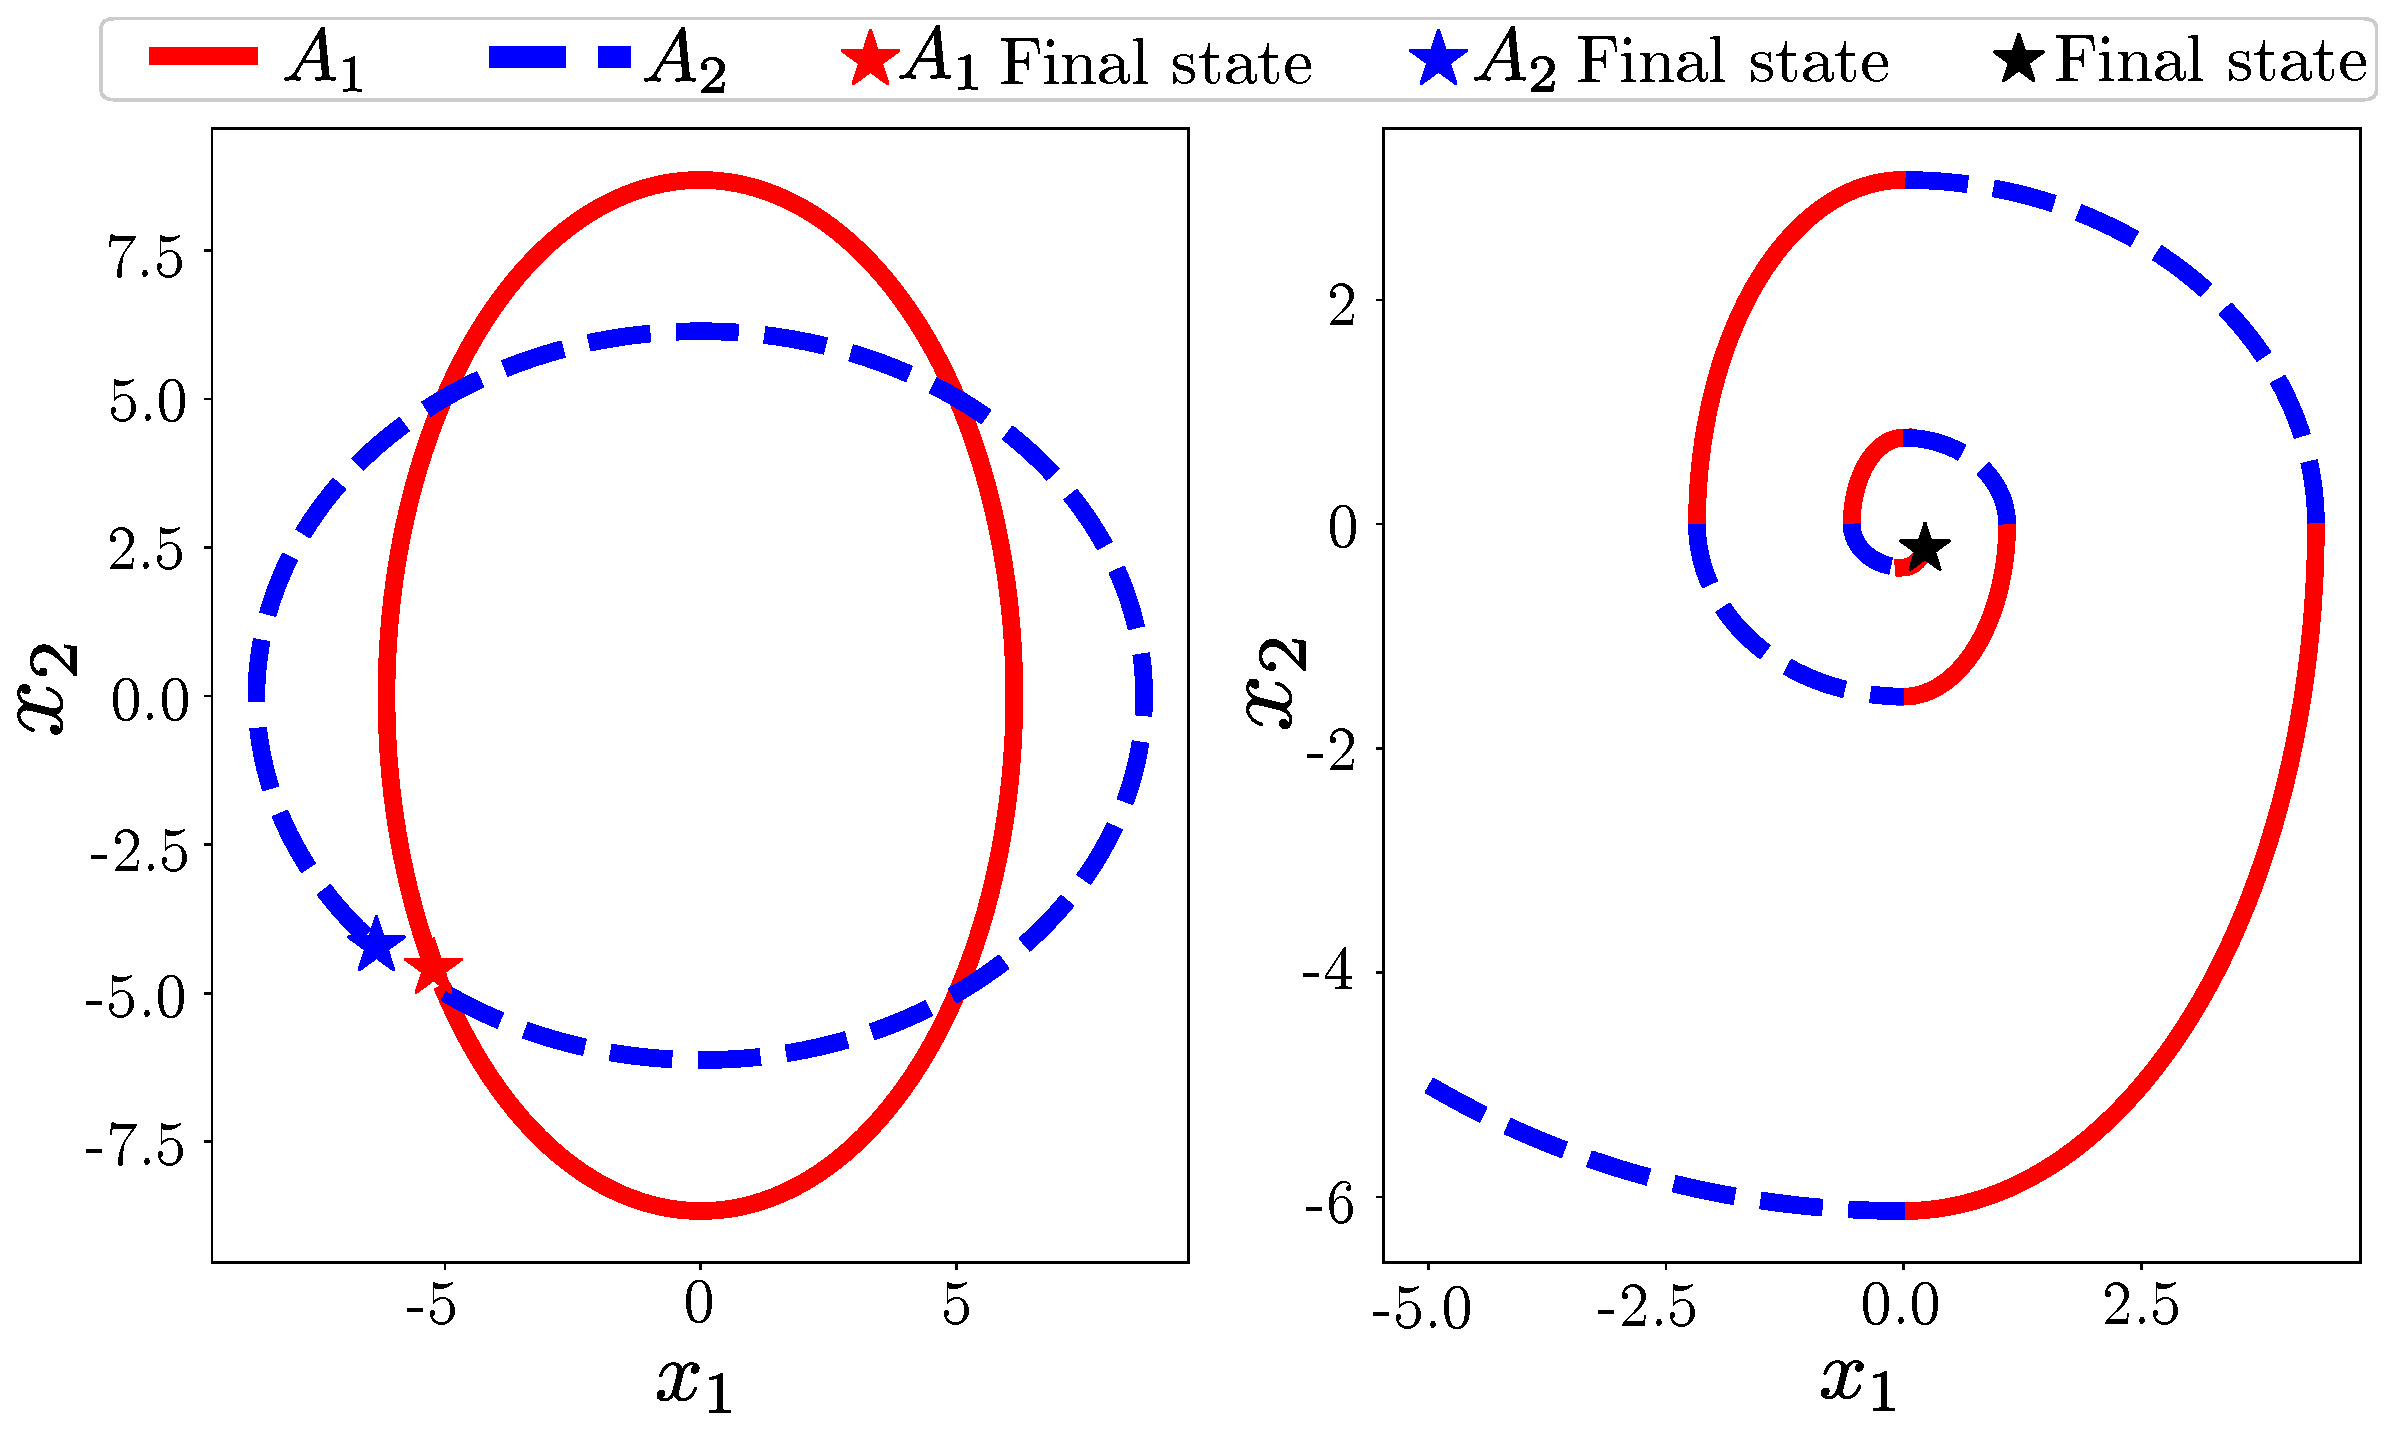
\includegraphics[width=0.7\linewidth]{switching_linear.eps}
    \subfloat[\label{marginally_stable}Two marginally stable closed-loop systems]{\hspace{0.5\linewidth}}
    \subfloat[\label{stable_switching}Asymptotically stable switching]{\hspace{0.5\linewidth}}
    \caption{Stable switching between two marginally stable systems }
    \label{fig:stableSwitching}
\end{figure}

Akin to the regression problem in Section~\ref{ssec:mixture_of_experts}, the
training dataset consists of \textit{input state-label} pairs, where the labels are
the performances of the trajectories generated under the current control law.
% 
In the case of the switching-control problem, we generate a trajectory and the
corresponding performance metric (labels) as follows.
%
Starting from some initial state $x(t=0)$, we sample a state partition index $i$
from the categorical distribution, whose probabilities are provided by the
gating network:
\begin{align}
    i  \sim \text{Categorical} (\mathbf{P}(x(t)| \psi)).
    \label{eq:gating_categorical}
\end{align} 
Given the partition index $i$, the expert (control law) is given by a sample
from the Bernoulli probability distribution
\begin{align}
    F_i(\theta_i) = \begin{cases}
       0, & \theta_i > \frac{1}{2}, \\
       1, & \theta_i \leq \frac{1}{2},
    \end{cases}
    \label{eq:bernoulli}
\end{align}
\noindent where $F_i = 0$ corresponds to the first dynamics $\dot{x} = A_1 x$
and $F_i=1$ corresponds to $\dot{x} = A_2x$. The parameter $\theta_i$ of the
expert is to be learned, and it determines which of the two experts to
execute in each partition.
%
In order to ensure that the parameter $\theta_i$ of the expert serves as the
probability of the Bernoulli distribution, we use the \textsc{Sigmoid}
function\cite{sharma2017activation} to limit $\theta_i$ between 0 and 1.
%
The next state $x(t+\Delta t)$ in the trajectory is obtained from the following
integration scheme:
\begin{align*}
    x(t + \Delta t) = (1-F_i) A_1 x(t) + F_i A_2 x(t).
\end{align*}
%
We repeat this process to generate a trajectory for the time-horizon $T$.
%
The performance of the trajectory generated under the current parameters $(\psi,
\theta)$ can be quantified by the metric $\ell$ as
\begin{align*}
    \ell(x(t + \Delta t)) := \frac{1}{2} \norm{x(t + \Delta t)}{}^2.
\end{align*}
In Section~\ref{ssec:performance_objective}, we generalize the performance
metrics to be applicable to various dynamical systems and discuss how we can
encode desired characteristics of the controller.
%
From the performance metric $\ell$, we can construct the cost function
$\mathbb{L}$ similar to the standard MoE framework
in~\eqref{eq:log_normal_likelihood} as
\begin{align*}
    \mathbb{L} \Bigl(\{x(0), \dots, x(T)\} \Bigr)= \sum_{t=0}^{T} \sum_{i=1}^{N_F} \ell_i \Bigl(x_i(t + \Delta t) \Bigr) \; P_i \Bigl(x(t), \psi \Bigr) .
\end{align*}
\noindent In the upcoming sections, we generalize the MoE control-search
problem and provide techniques to efficiently learn the optimal decision
parameters from appropriate cost functions.


\section{Mixture of Experts Controller}
\label{sec:moe_methods}

Based on the motivating example provided in
Section~\ref{sec:motiviational_application}, we present a generalized
data-driven control design framework for hybrid dynamical systems.
%
In this framework, the controller is given by deep-net mixture of experts
$F(x;\theta)$, and the control switching scheme is governed by the gating
network $\mathbf{P}(x|\psi)$.
%
This technique allows us to observe the effects of mode changes from the
closed-loop trajectories and learn a switching mechanism to best control the
hybrid system across modes.
%
The objective is to learn the parameters $\theta_i$ of each expert and the
gating network $\psi$ that can achieve the desired performance.


%
Let $\phi(x_0, u, T)$ denote a closed-loop trajectory generated from a hybrid
dynamical model starting from initial state $x_0$.
%
For every state $x$ in a trajectory, the control law first samples a state
partition index $i$ from a categorical distribution and evaluates the
corresponding expert as
\begin{align}
    u(x; \psi, \theta) = \{F_i&(x; \theta_i) \; | \; i  \sim \text{Categorical} (\mathbf{P}(x| \psi)) \}.
    \label{eq:categorical}
\end{align} 
%
We use the metric $\ell : \mathcal{X} \times \mathcal{U} \rightarrow
\mathbb{R}$ to measure the performance of the sampled experts, which we discuss
in depth in Section~\ref{ssec:performance_objective}.
%
% The running cost plays the role of \it{prediction error} \normalfont in the
% construction of the cost function $\mathcal{L}$ as shown
% in~\eqref{eq:original_normal_likelihood}.
%
The goal is to learn the decision parameters $(\psi, \theta)$ that minimize the
metric $\ell$ for all initial states in the state space.
%
We pose the search over the parameters of the experts and the gating network as the following optimization problem.
\begin{equation}
    \begin{aligned}
        \underset{\psi, \theta}{\textrm{minimize}} 
        & & &\int_0^T \ell (x(t),u) \dd t , \\%
        \textrm{subject to}
        & & M(q) &\dd \dot{q} + h(q, \dot{q})\dd t - \dd R  = 0\\%
        & & u = \{F_i&(x; \theta_i) \; | \; i  \sim \text{Categorical} (\mathbf{P}(x| \psi)) \}.
    \end{aligned}
    \label{eq:moe_opt}
\end{equation}
%
In Section~\ref{ssec:training_moe}, we provide a procedure to solve the
optimization problem~\eqref{eq:moe_opt} via stochastic gradient descent. 
\begin{rem}
    Without prior knowledge injected to the gating network, the samples from the
    categorical distribution in~\eqref{eq:categorical} initially explore the
    performance of most, if not all, of the expert controllers.
    %
    As the parameters converge to their optimal values, the samples from the
    categorical distribution correspond to the indices of the single best
    experts and the control law in~\eqref{eq:categorical} is equivalent
    to~\eqref{eq:best_expert_prediction}.
\end{rem}

\subsection{Performance Metrics}
\label{ssec:performance_objective}
%
We present two viable choices for the performance metric $\ell$. 
\begin{enumerate}
    \item \textbf{Accumulated cost}: is the total quadratic loss between the
    desired state $x^*$ and the states generated under the current control law.
    We can also enforce control saturations for underactuated systems by incurring a
    cost on the control input as follows:
    \begin{equation}
        \begin{gathered}
            \ell(x, u) = \frac{1}{2}(x - x^*)^\top \mathcal{Q} (x - x^*) + \frac{1}{2} u^\top \mathcal{R} u , 
            % \ell(\phi, u) = \int_0^{T}  \ell(x(t), u)\dd t,
        \end{gathered}
    \label{eq:accumulatedLoss}
    \end{equation}
    \noindent where $\mathcal{Q} \succ 0$ denotes a positive definite matrix and
    $\mathcal{R} \succeq 0$ represents a positive semi-definite matrix.
    %
    This construction encourages trajectories to reach the desired equilibrium
    with minimum effort and shortest time.
    %
    We modify the cost function $\mathbb{L}$ presented
    in~\eqref{eq:log_normal_likelihood} to incorporate the quadratic loss
    $\ell(x, u)$ as follows:
    \begin{align}
        \mathbb{L}(\phi) = \sum_{t=0}^{T} \sum_{i=1}^{N_F} \ell_i \Bigl(x_i(t+\Delta t), F_i \Bigr) P_i\Bigl(x(t) | \psi \Bigr)  .
        \label{eq:accumulated_likelihood}
    \end{align}
    %
    % The quadratic loss in~\eqref{eq:accumulatedLoss} plays the role of prediction
    % error in~\eqref{eq:original_normal_likelihood}.
    %
    Similar to the regression problem provided in
    Section~\ref{ssec:mixture_of_experts}, the accumulated
    cost~\eqref{eq:accumulated_likelihood} is minimum when the metric $\ell_i$
    achieved by expert $i$ is low and the responsibility $P_i(x(t) | \psi)$ of
    the expert is high.
    %

    %
    Algorithm~\eqref{algo:accumulated_loss} outlines how we construct the
    cost function from a trajectory.
    %
    In this procedure we check the performance of each expert at every
    integration step.
    %
    To do so, starting at initial state $x_0$, we integrate the dynamics
    in~\eqref{eq:hybrid_dynamics} for one time step $\Delta t$ using all the
    experts in $F(x_0;\theta)$.
    %
    We retrieve all the states $\{ x_i(\Delta t) , i \in \{1, \dots N_F \}\}$
    obtained from the integration and evaluate the running cost $\ell(x_i(\Delta
    t), F_i)$ incurred by each expert.
    %
    Each performance metric $\ell(x_i(\Delta t), F_i)$ is weighed by its
    \textit{responsibility} $P_i(x_0 | \psi)$ and summed across experts to get
    the cost function.
    \begin{algorithm}[tb]
        \setstretch{1.2}
        \caption{Accumulated Cost}
        \label{algo:accumulated_loss}
        \small
        \hspace*{\algorithmicindent} \textbf{Input}: $x_0, \theta, \psi$
        \begin{algorithmic}[1]
            \State $\mathbb{L} \leftarrow 0$
            % \algrenewcommand\algorithmicindent{0em} % No indent
                \For{$t = 0:\Delta t:T$}     
                \For{$j=1:N_F$}\Comment{Evaluate performance of each expert}
                    \State $x_j(t+\Delta t) \leftarrow \texttt{Moreau's one time step}(x(t), F_j(x(t), \theta_j))$\Comment{Algorithm~\eqref{algo:moreau}}
                    \State $\mathbb{L} \leftarrow \mathbb{L} - \ell(x_j(t+\Delta t), F_j) \; P_j(x(t) | \psi)$
                \EndFor
                \State $i \sim \text{Categorical}\Bigl(\mathbf{P}(x(t)| \psi)\Bigr)$ \Comment{Sample a bin number}
                \State $x(t + \Delta t) \leftarrow \texttt{Moreau's one time step}(x(t), F_i(x(t), \theta_i))$
                \EndFor
            \State \textbf{return} $\mathbb{L}$
        \end{algorithmic}
    \end{algorithm}
    %
    By checking the performance of each expert for every state, the computation
    of the cost function is prone to the curse of dimensionality.
    %
    We minimize the amount of computation needed to compose the cost function by
    selecting one state from the collection $\{ x_i(\Delta t) , i \in \{1,
    \dots N_F \}\}$ to continue the integration.
    %
    We select the expert responsible for generating the next state $x(\Delta t)$
    from the categorical distribution~\eqref{eq:categorical}.
    %
    This process is repeated for every time step in the trajectory.
    % Notice that for each state $x(t)$, we need to test the performance of each expert. 
    % %
    % For instance, if there are $100$ states in a trajectory and $3$ experts, we need to evaluate $\ell$ $300$ times.

    \begin{rem}    
        Notice that the accumulated cost checks the performance of each expert at
        every state.
        %
        When training for few experts, this cost function provides ample
        exploration, resulting in fast convergence to an optimal control strategy.
        %
        However, for numerous experts, the accumulated cost incurs large
        computational overhead.
    \end{rem}

    \item \textbf{Minimum trajectory loss (MTL)}: is designed to minimize the
    computational complexities of the accumulated cost.
    %
    Compared to~\eqref{eq:accumulated_likelihood}, MTL may also better represent
    the desired behavior of some dynamical systems.
    %
    Consider the classical control problem of swinging-up the simple pendulum to
    the upright equilibrium. 
    %
    For an underactuated pendulum, a successful controller needs to swing the
    pendulum clockwise and counterclockwise, passing through the downward
    equilibrium point multiple times until enough kinetic energy is built up to
    reach the upward equilibrium.
    %
    Accumulated loss incurs high cost in such scenarios and the control
    search would get stuck in a local minimum.
    %
    In such cases, a successful cost function encourages trajectories that
    \textit{eventually} lead to the goal state.
    %
    This is achieved by MTL, which is composed of the lowest cost incurred
    across the entire trajectory and the responsibilities of the experts that
    led to the minimum cost.
    %
    The resulting cost function $\mathbb{L}$ is given by
    \begin{equation}
        \begin{gathered}
            t_{\text{min}} = \underset{t}{\textrm{inf}} \; \{ \ell(x(t), u): x(t) \in \phi(x_0, u, T) \},  \\
            \mathbb{L}(\phi) = \frac{\ell(x(t_{\text{min}}), u)}{C} \sum_{t=0}^{t_{\text{min}}}P_i(x(t) | \psi), 
        \end{gathered} 
    \end{equation}
    \noindent where $C > 0$ is a normalization factor.
    %
    The detailed procedure for the construction of MTL is shown in
    Algorithm~\eqref{algo:mtl}.
    %
    Unlike the accumulated cost, MTL does not particularly reward low effort or
    short time trajectories, but it equally rewards two trajectories
    as long as they both reach the goal state within the time horizon $T$. 
    %
    \begin{algorithm}[tb]
        \setstretch{1.2}
        \caption{Minimum Trajectory Loss}
        \label{algo:mtl}
        \small
        \hspace*{\algorithmicindent} \textbf{Input}: $x_0, \theta, \psi$
        \begin{algorithmic}[1]
            % \algrenewcommand\algorithmicindent{0em} % No indent
            \State $\phi \leftarrow \{ x_0 \}$
                \For{$t = 0:\Delta t:T$}     
                    \State $i \sim \text{Categorical}\Bigl(\mathbf{P}(x(t)| \psi)\Bigr)$ \Comment{Sample a bin number}
                    \State $x(t + \Delta t) \leftarrow \texttt{Moreau's one time step}(x(t), F_i(x(t), \theta_i))$\Comment{Algorithm~\eqref{algo:moreau}}
                    \State $\phi \leftarrow \phi \cup x(t+\Delta t)$
                \EndFor
                \State $t_{min} = \underset{t}{\textrm{inf}} \; \{ \ell(x(t), u): x(t) \in \phi\}$
                \State $\mathbb{L} = - \ell(x(t_{min}), u) \sum_{t=0}^{t_{min}}P_i(x(t) | \psi)  $
            \State \textbf{return} $\mathbb{L}$
        \end{algorithmic}
    \end{algorithm}
\end{enumerate}

\subsection{State Sampling}
\label{ssec:state_sampling}

We intend to find a solution to the optimization problem
in~\eqref{eq:moe_opt} for all initial states $x_0$ in the
state space.
%
To do so, we generate the performance metric $\ell$ from \textit{a batch of
initial states} and update the parameters $(\psi, \theta)$ \textit{iteratively}
via stochastic gradient descent (SGD). 
%
To efficiently sample the initial states, we use a combination of greedy and
explorative state sampling techniques.
%
An example of greedy state sampling technique, commonly known as \textit{Dataset
Aggregation} (\textsc{DAgger}), is a technique adapted from imitation
learning~\cite{ross2011no}.
%
This method collects states most visited under the current parameters $(\psi,
\theta)$ and concentrates on refining the performance of the controller on these
states.
%
For instance, suppose we are solving the optimization in~\eqref{eq:moe_opt} to
obtain a controller that swings up an underactuated simple pendulum to the
upright.
% %
Initially, the parameters $(\psi, \theta)$ may result in a controller that
swings the pendulum to the downward equilibrium irrespective of where it
started.
%
Thus, it is most efficient to first expose the training to the cost incurred by
visiting the downward equilibrium.
%
In this technique, we first discretize the state space and uniformly sample
several initial states.
%
Starting from those initial states, we generate trajectories using the current
parameters.
%
In order to improve the controller at the states favored by the current policy,
we draw $N_d$ initial state samples from the states visited in the trajectories. 
%
At first, the $N_d$ samples mostly consist of states near the downward equilibrium.
%
As the parameter update continues, \textsc{DAgger} starts sampling states that
are closer to the upright equilibrium.
%
This efficient state exposition is pivotal for the convergence to the optimal
parameters.



The explorative state sampling technique exposes the training to the rewards of
approaching and remaining close to $x^*$.
%
It also uses random sampling to explore new control strategies and recover from locally optimal
solutions.  
%
This method collects $N_r$ initial states around the neighborhood of the desired
equilibrium by drawing samples from the normal distribution $x_0 \sim \mathcal{N}(x^*, \delta)$,
whose mean is $x^*$ and the standard deviation is a small constant $\delta$.
%
For each parameter update in SGD, we compute the performance metric as an expectation
over $N_{\mathcal{D}} = N_d+N_r$ samples as follows:
\begin{align}
    J(\phi, u) = \mathbb{E}_{x_0 \in \mathcal{D}_N}[ \mathbb{L}(\phi(x_0, u, T))],
    \label{eq:average_cost}
\end{align}
\noindent where $\mathcal{D}_N$ is a \textit{replay buffer} consisting of
$N_{\mathcal{D}}$ initial state samples.


\subsection{Training Mixture of Experts Controller}
\label{ssec:training_moe}

%
We solve the optimization problem in~\eqref{eq:moe_opt} following the procedure
outlined in Algorithm~\eqref{algo:moe_training}.
%
At the beginning of the training, we collect $N_{\mathcal{D}}$ initial states
samples using the greedy and explorative state sampling techniques discussed in
Section~\ref{ssec:state_sampling} and save them in the replay buffer $\mathcal{D}_N$.
%
For every initial state in the replay buffer, we generate a trajectory using the
current decision parameters $(\psi, \theta)$ and assign the cost function
$\mathbb{L}$.
%
The average cost incurred by the current policy is given by $J$
in~\eqref{eq:average_cost}, from which we compute the pertinent gradients
$\nicefrac{\partial J}{\partial \psi}, \nicefrac{\partial J}{\partial \theta}$
via auto-differentiation techniques.
%
In particular, we use forward-mode auto-differentiation~\cite{revels2016forward}
to take the gradient through the trajectory generated from Moreau's integration
scheme.
%
Although not explored in this work, it is possible to design adjoint methods for
hybrid systems to efficiently back-propagate on the cost function through
reverse-mode auto-differentiation techniques.
%
We invoke a variant of stochastic gradient descent known as
\textsc{Adam}~\cite{kingma2014adam} to efficiently update the parameters with
adaptive learning rates $\alpha$.
%
\begin{algorithm}[tb]
    \setstretch{1.2}
      \caption{Solution to the MoE Optimization Problem~\eqref{eq:moe_opt}}
      \label{algo:moe_training}
      \small
      \begin{algorithmic}[1]
          \algrenewcommand\algorithmicindent{0em} % No indent
          \State $\mathcal{D}_N \gets \{x_0\}_{(N_{\mathcal{D}})}$  \Comment{$N_{\mathcal{D}}$ initial state samples} 
          \algrenewcommand\algorithmicindent{1.1em} % Change indent back to default
          \While{$i < $ \texttt{maximum iteration}}
          \State $J \gets 0$\Comment{Batch loss}
          \For{$x_0 \in \mathcal {D}_N$}
              \State $\mathbb{L}$ = \texttt{Performance objective}($x_0, \psi, \theta$) \Comment{Algorithm~\eqref{algo:accumulated_loss} or~\eqref{algo:mtl}}
              \State $J \gets J + \mathbb{L}/N_{\mathcal{D}}$ 
          \EndFor
          \State $\theta \gets \theta - \alpha \nicefrac{\partial J}{\partial \theta}$\Comment{SGD step}
          \State $\psi \gets \psi - \alpha \nicefrac{\partial J}{\partial \psi}$
          \State $\mathcal{D}_N \gets \{x_0\}_{(N_{\mathcal{D}})}$\Comment{New initial state samples}
          \State $i \;\:\gets i + 1$
          \EndWhile
          \State \textbf{return} $\theta$
      \end{algorithmic}
\end{algorithm}
%

\subsection{Back-propagation through Hybrid Dynamics}
\label{ssec:backprop_hybrid}

The training framework outlined~\eqref{eq:moe_opt} allows us to observe the
effects of contacts in the closed-loop trajectories and infer a controller that
either uses the contact to its advantage or minimizes its adverse effects.
%
In this section, we look at the relevant parts of the back-propagation to give
insight on how this is achieved.
%
We also show that despite the state jumps in the hybrid dynamics, the
derivatives involved in the back-propagation are well-defined.

Suppose we generate a short trajectory $\phi$ with the sampled expert control
parameter $\theta_i$.
%
Forward-mode auto-differentiation evaluates the gradient of the accumulated cost
with respect to $\theta_i$ as 
\begin{align*}
    \frac{\partial \ell}{\partial \theta_i} = \sum_{t=0}^{T} \frac{\partial \ell}{\partial x_t} \frac{\partial x_t}{\partial \theta_i} ,
\end{align*}
\noindent where $R=0$ for simplicity.
%
Without loss of generality, we take one integration step for the reminder of
this discussion. 
%
In that step, a contact event is triggered causing the velocities to jump
between the initial state $x_0$ and the following state $x_1$. 
%
Hence, we focus on 
\begin{align*}
    \frac{\partial \ell}{\partial \theta_i} = \frac{\partial \ell}{\partial x_1} \frac{\partial x_1}{\partial \theta_i},
\end{align*}
%
We can expand the gradient further as 
\begin{align*}
    \frac{\partial \ell}{\partial \theta_i} = \frac{\partial \ell}{\partial x_1} \Bigl( \frac{\partial x_1}{\partial u} \frac{\partial u}{\partial \theta_i} + \frac{\partial x_1}{\partial \lambda}\frac{\partial \lambda}{\partial \theta_i}\Bigr),
\end{align*}
\noindent where $\lambda=[\lambda_N, \lambda_T]$ holds the contact forces.
%
We can compute the first term from Moreau's integration step as
\begin{align*}
    \frac{\partial x_1}{\partial u} \frac{\partial u}{\partial \theta_i} = 
    \bmat{M^{-1}B \Delta t^2/2 \\ M^{-1}B \Delta t} \frac{\partial u}{\partial \theta_i},
\end{align*} 
%
At first glance, it may seem the derivative $\frac{\partial x_1}{\partial
\lambda}\frac{\partial \lambda}{\partial \theta_i}$ does not exist due to
the discontinuity in the states. 
%
A closer observation reveals that  $\frac{\partial x_1}{\partial \lambda}$
determines how the \it{post-impact velocity is affected by the
contact forces}.~\normalfont
%
In fact, the derivative can be found from Moreau's integration as 
\begin{align*}
    \frac{\partial x_1}{\partial \lambda} = \bmat{W_N & W_T }, 
\end{align*}
%
demonstrating that the gradient exists even if a state jump has occurred. 
%
This term is crucial in adjusting the decision parameters in response to how the
contact force assists or inhibits the system.
%
If the contact forces affect the \it{post-impact} \normalfont velocity such that
the resulting generalized coordinates are closer to the desired state $x^*$,
then the gradient $\frac{\partial \ell}{\partial x_1} \frac{\partial
x_1}{\partial \lambda}\frac{\partial \lambda}{\partial \theta_i}$ adjusts the
parameter $\theta_i$ to favor states undergoing contact events. 
%
Indeed, we demonstrate this behavior in simulation and real-world experiments in
Section~\ref{ssec:cartpole_with_walls}.
%
Conversely, if the contact forces move the states further away from $x^*$, the
gradient leads to control parameters that attempt to recover from the outcomes
of the contact events.
%
We also demonstrate this behavior on a walking robot example in
Section~\ref{sssec:rimless_wheel_model}.
